%% OVERVIEW
Experiments are divided into three parts\footnote{Details on network architectures, training parameters as well as more experiments are included in the supplementary material.}. First we compare with state-of-the-art methods for 3D object detection on KITTI~\cite{geiger2013vision} and SUN-RGBD~\cite{song2015sun} (Sec~\ref{sec:exp_benchmark}). Second, we provide in-depth analysis to validate our design choices (Sec~\ref{sec:exp_analysis}). Last, we show qualitative results and discuss the strengths and limitations of our methods (Sec~\ref{sec:exp_viz}).

% \subsection{Implementation Details and Training}
% loss weight. data augmentation. optimizer, learning rate schedule, training time and hardware etc.

%% KITTI and SUN-RGBD
\subsection{Comparing with state-of-the-art Methods} \label{sec:exp_benchmark}
We evaluate our 3D object detector on KITTI~\cite{Geiger2012CVPR} and SUN-RGBD~\cite{song2015sun} benchmarks for 3D object detection. On both tasks we have achieved significantly better results compared with state-of-the-art methods.

%2d AP, birdeye AP and 3D AP on both validation set and test set. report speed as well.
%[optional] show how bird-eye view proposal can help?

\paragraph{KITTI} Tab.~\ref{tab:kitti_test_3d_detection} shows the performance of our 3D detector on the KITTI \emph{test} set. We outperform previous state-of-the-art methods by a large margin. While MV3D~\cite{cvpr17chen} uses multi-view feature aggregation and sophisticated multi-sensor fusion strategy, our method based on the PointNet~\cite{qi2017pointnet} (v1) and PointNet++~\cite{qi2017pointnetplusplus} (v2) backbone is much cleaner in design. While out of the scope for this work, we expect that sensor fusion (esp. aggregation of image feature for 3D detection) could further improve our results.

We also show our method's performance on 3D object localization (bird's eye view) in Tab.~\ref{tab:kitti_test_3d_localization}. In the 3D localization task bounding boxes are projected to bird's eye view plane and IoU is evaluated on oriented 2D boxes. Again, our method significantly outperforms previous works which include DoBEM~\cite{yuvehicle} and MV3D~\cite{cvpr17chen} that use CNNs on projected LiDAR images, as well as 3D FCN~\cite{li20163d} that uses 3D CNNs on voxelized point cloud. 
%We also compare with two unpublished methods (AVOD and NVLidarNet) that are available on the KITTI leader board~\cite{kitti-3d-localization}.

The output of our network is visualized in Fig.~\ref{fig:results} where we observe accurate 3D instance segmentation and box prediction even under very challenging cases. We defer more discussions on success and failure case patterns to Sec.~\ref{sec:exp_viz}. We also report performance on KITTI val set (the same split as in~\cite{cvpr17chen}) in Tab.~\ref{tab:kitti_val_3d_detection} and Tab.~\ref{tab:kitti_val_3d_localization} (for cars) to support comparison with more published works, and in Tab.~\ref{tab:val_ped_cyc} (for pedestrians and cyclists) for reference.

%The object detection benchmark in KITTI provides synchronized RGB images and LiDAR point clouds with groundtruth amodal 2D and 3D box annotations for vehicles, pedestrians and cyclists. The training set contains 7481 frames and a undisclosed test set contains 7581 frames. In our own experiments we follow ~\cite{chen2016monocular,cvpr17chen} to split the official training set to a train set of 3717 frames and a val set of 3769 frames such that frames in train/val sets belong to different video clips. Objects in KITTI are also categorized into different difficulty levels (easy, medium and hard) depending on its size in image and its truncation and occlusion levels.



\begin{table}[t!]
\small
\centering
\label{tab:kitti_valid}
\begin{tabular}{l||ccc}
\hline
Method & Easy    & Moderate    & Hard   \\ \hline
Mono3D~\cite{chen2016monocular} & 2.53 & 2.31 & 2.31 \\ %\hline
3DOP~\cite{chen20153d}  & 6.55 & 5.07 & 4.10 \\ \hline
VeloFCN~\cite{li20163d} & 15.20 & 13.66 & 15.98 \\ %\hline
MV3D (LiDAR)~\cite{cvpr17chen} & 71.19 & 56.60 & 55.30 \\ %\hline
MV3D~\cite{cvpr17chen} & 71.29 & 62.68 & 56.56 \\ \hline
Ours (v1) & 83.26 & 69.28 & 62.56 \\
Ours (v2) & \textbf{83.76} & \textbf{70.92} & \textbf{63.65}\\ \hline
\end{tabular}
\caption{\textbf{3D object detection} AP on KITTI \emph{val} set (cars only).}
\label{tab:kitti_val_3d_detection}
\end{table}


\begin{table}[t!]
\small
\centering
\label{tab:kitti_valid}
\begin{tabular}{l||ccc}
\hline
Method & Easy    & Moderate   & Hard   \\ \hline
Mono3D~\cite{chen2016monocular} & 5.22 & 5.19 & 4.13 \\ %\hline
3DOP~\cite{chen20153d}  & 12.63 & 9.49 & 7.59 \\ \hline
VeloFCN~\cite{li20163d} &  40.14 & 32.08 & 30.47 \\ %\hline
MV3D (LiDAR)~\cite{cvpr17chen} & 86.18 & 77.32 & 76.33 \\ %\hline
MV3D~\cite{cvpr17chen} & 86.55 & 78.10 & \textbf{76.67} \\ \hline
Ours (v1) & 87.82 & 82.44 & 74.77 \\
Ours (v2) & \textbf{88.16} & \textbf{84.02} & 76.44 \\ \hline
\end{tabular}
\caption{\textbf{3D object localization} AP on KITTI \emph{val} set (cars only).}
\label{tab:kitti_val_3d_localization}
\end{table}

\begin{table}[h!]
\small
\centering
\begin{tabular}{|c|c|c|c|}
    \hline
    Benchmark & Easy & Moderate & Hard \\ \hline
    Pedestrian (3D Detection) & 70.00 & 61.32 & 53.59 \\ \hline
    Pedestrian (Bird's Eye View) & 72.38 & 66.39 & 59.57 \\ \hline
    Cyclist (3D Detection) & 77.15 & 56.49 & 53.37 \\ \hline
    Cyclist (Bird's Eye View) & 81.82 & 60.03 & 56.32 \\ \hline
\end{tabular}
\caption{Performance on KITTI \emph{val} set for pedestrians and cyclists. Model evaluated is Ours (v2).}
\label{tab:val_ped_cyc}
\end{table}

\paragraph{SUN-RGBD} Most previous 3D detection works specialize either on outdoor LiDAR scans where objects are well separated in space and the point cloud is sparse (so that it's feasible for bird's eye projection), or on indoor depth maps that are regular images with dense pixel values such that image CNNs can be easily applied. However, methods designed for bird's eye view may be incapable for indoor rooms where multiple objects often exist together in vertical space. On the other hand, indoor focused methods could find it hard to apply to sparse and large-scale point cloud from LiDAR scans.

In contrast, our frustum-based PointNet is a generic framework for both outdoor and indoor 3D object detection. By applying the same pipeline we used for KITTI data set, we've achieved state-of-the-art performance on SUN-RGBD benchmark (Tab.~\ref{tab:sunrgbd}) with significantly higher mAP as well as much faster (10x-1000x) inference speed.

%While 2D-driven~\cite{lahoud20172d} also uses 2D detector proposals and then estimate 3D bounding box in frustum point cloud, they rely on hand-crafted features in point cloud that are not only sub-optimal in performance and speed but also hard to generalize to outdoor cases with widely distributed points in space.

%The data set consists of 10,355 RGB-D images captured from various depth sensors for indoor scenes (bedrooms, dining rooms etc.). We follow the same train/val splits as \cite{song2015sun,ren2016three} for experiments and report our method's result with v1 models in Table~\ref{tab:sunrgbd}.


\begin{figure*}[t!]
    \centering
    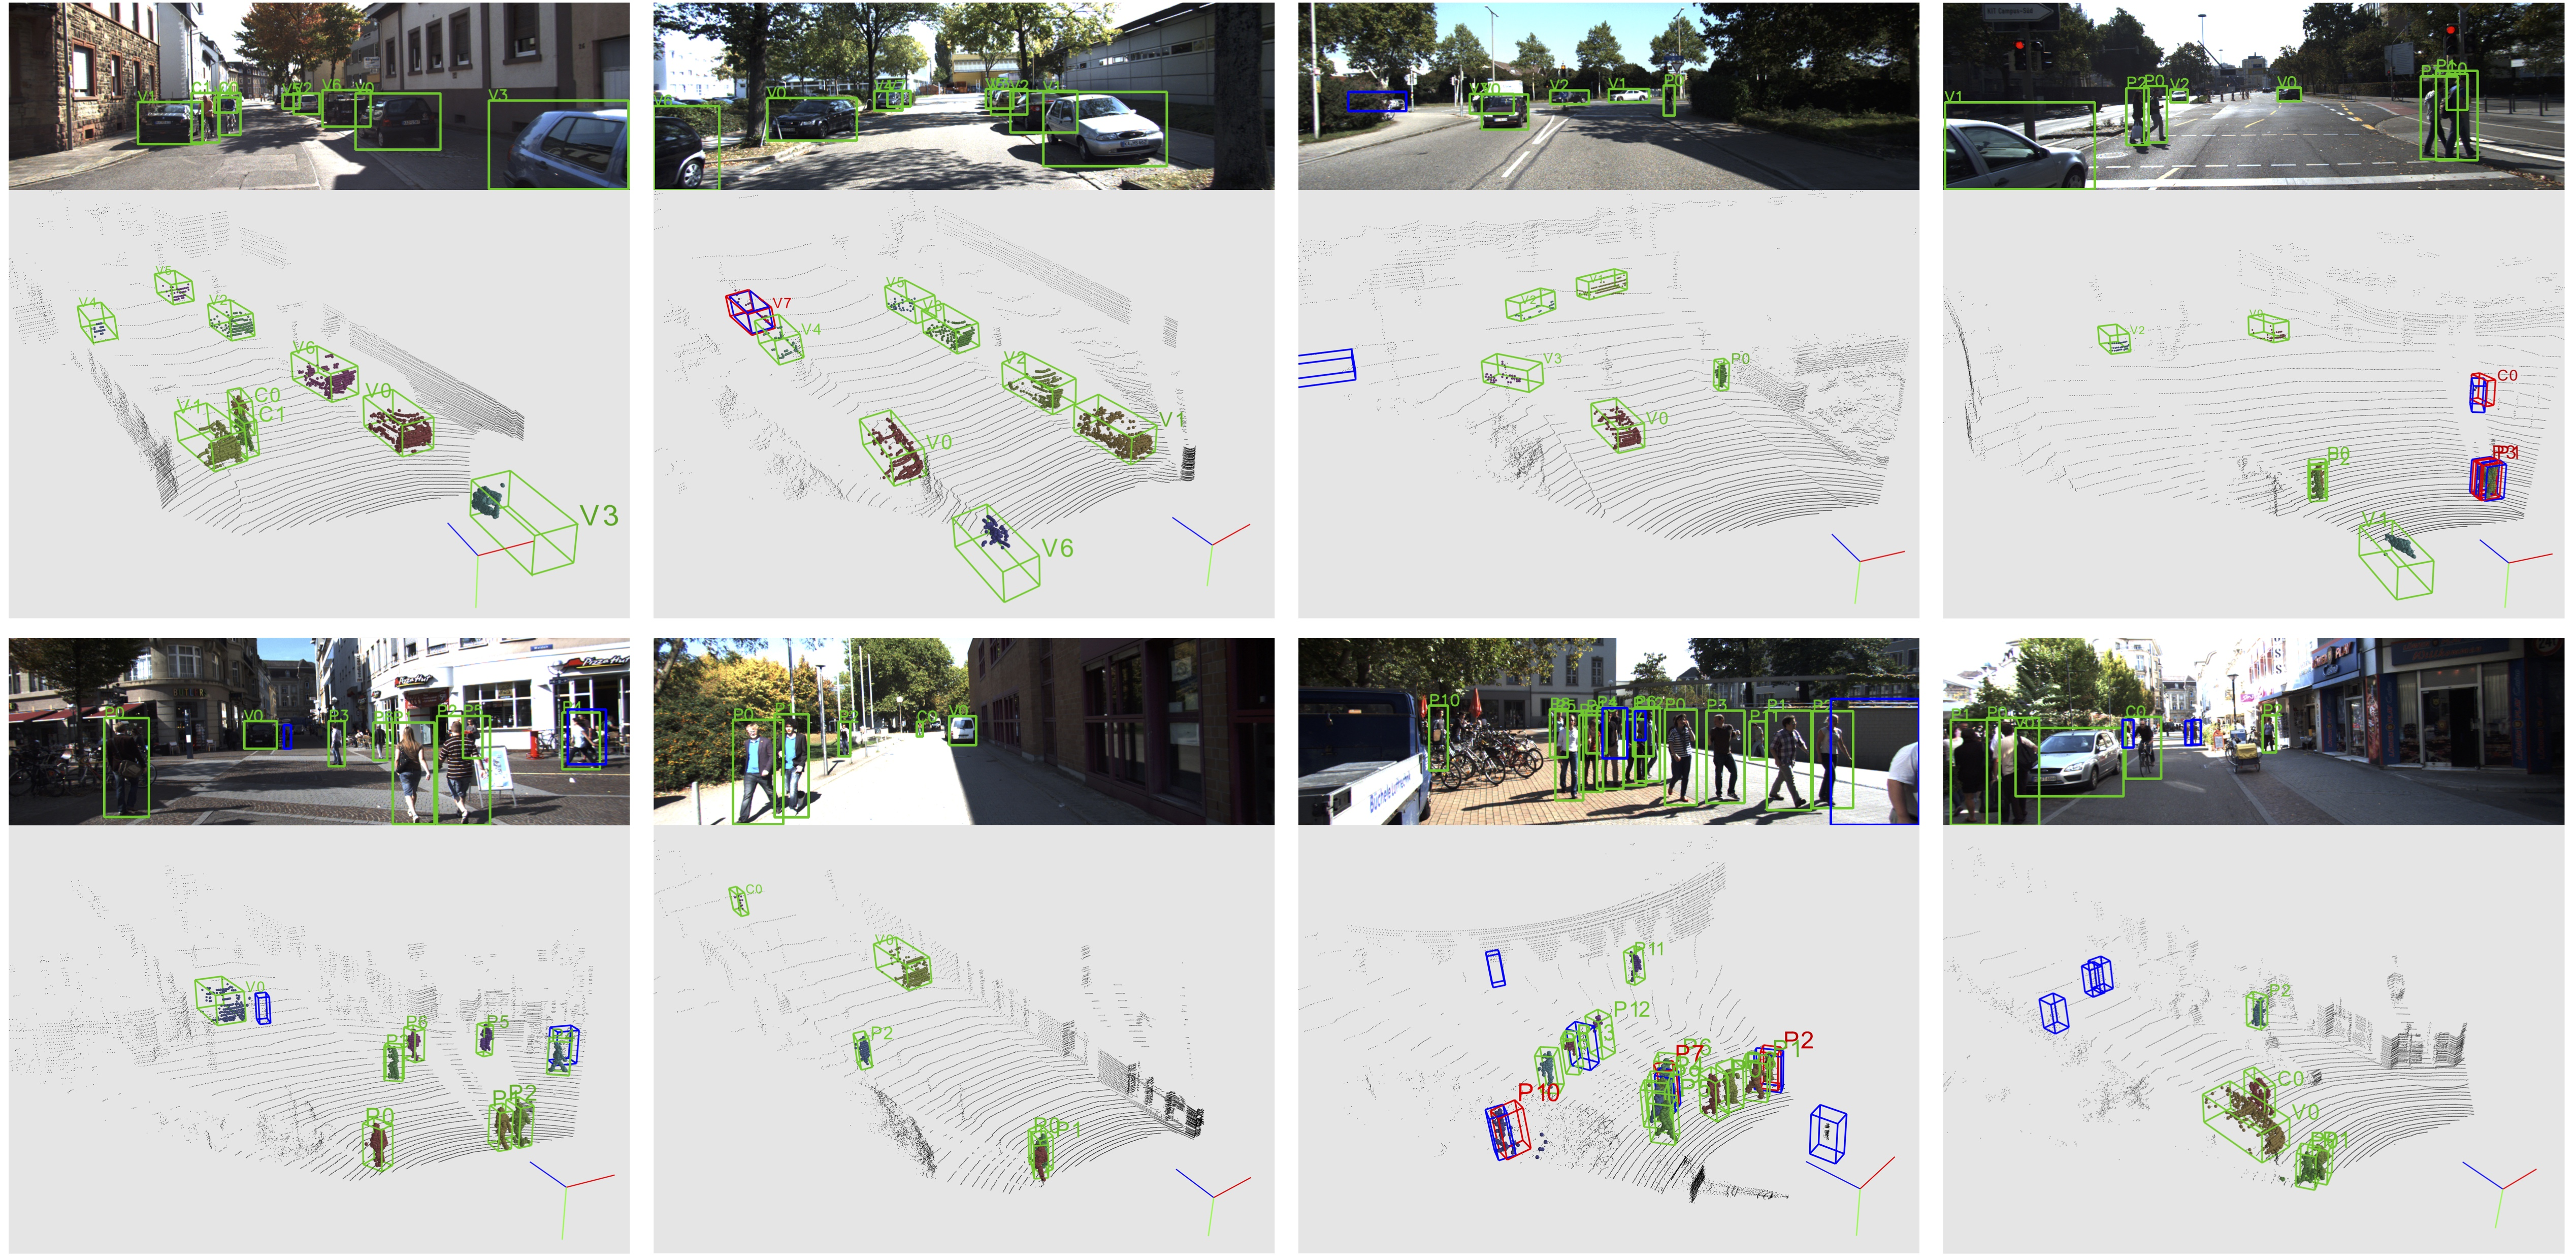
\includegraphics[width=\linewidth]{fig/results.jpg}
    \caption{\textbf{Visualizations of Frustum PointNet results on KITTI val set}  (best viewed in color with zoom in). These results are based on PointNet++ models~\cite{qi2017pointnetplusplus}, running at 5 fps and achieving test set \emph{3D} AP of 70.39, 44.89 and 56.77 for car, pedestrian and cyclist, respectively. 3D instance masks on point cloud are shown in color. True positive detection boxes are in green, while false positive boxes are in red and groundtruth boxes in blue are shown for false positive and false negative cases. Digit and letter beside each box denote instance id and semantic class, with ``v'' for cars, ``p'' for pedestrian and ``c'' for cyclist. See Sec.~\ref{sec:exp_viz} for more discussion on the results.}
    \label{fig:results}
\end{figure*}

\begin{table*}[t!]
\small
\centering
\begin{tabular}{l|cccccccccc|c|c}
\hline
          & bathtub & bed & bookshelf & chair & desk & dresser & nightstand & sofa & table & toilet & Runtime  & mAP \\ \hline
DSS~\cite{song2016deep} & 44.2 & 78.8 & 11.9 & 61.2 & 20.5 & 6.4 & 15.4 & 53.5 & 50.3 & 78.9 & 19.55s   & 42.1    \\
COG~\cite{ren2016three} & \textbf{58.3} & 63.7 & 31.8 & 62.2 & \textbf{45.2} & 15.5 & 27.4 & 51.0 & \textbf{51.3} & 70.1 & 10-30min & 47.6 \\
2D-driven~\cite{lahoud20172d} & 43.5 & 64.5 & 31.4 & 48.3 & 27.9 & 25.9 & 41.9 & 50.4 & 37.0 & 80.4 & 4.15s    & 45.1  \\ \hline
Ours (v1) & 43.3 & \textbf{81.1} & \textbf{33.3} & \textbf{64.2} & 24.7 & \textbf{32.0} & \textbf{58.1} & \textbf{61.1} & 51.1 & \textbf{90.9} & 0.12s & \textbf{54.0} \\ \hline
\end{tabular}
\caption{\textbf{3D object detection AP on SUN-RGBD val set.} Evaluation metric is average precision with 3D IoU threshold 0.25 as proposed by~\cite{song2015sun}. Note that both COG~\cite{ren2016three} and 2D-driven~\cite{lahoud20172d} use room layout context to boost performance while ours and DSS~\cite{song2016deep} not. Compared with previous state-of-the-arts our method is 6.4\% to 11.9\% better in mAP as well as one to three orders of magnitude faster.}
\label{tab:sunrgbd}
\end{table*}


%% ANALYSIS EXPERIMENTS
\subsection{Architecture Design Analysis} \label{sec:exp_analysis}
In this section we provide analysis and ablation experiments to validate our design choices.

\paragraph{Experiment setup.} Unless otherwise noted, all experiments in this section are based on our v1 model on KITTI data using train/val split as in~\cite{cvpr17chen}. To decouple the influence of 2D detectors, we use ground truth 2D boxes for region proposals and use 3D box estimation accuracy (IoU threshold 0.7) as the evaluation metric. We will only focus on the car category which has the most training examples.

\paragraph{Comparing with alternative approaches for 3D detection.} In this part we evaluate a few CNN-based baseline approaches as well as ablated versions and variants of our pipelines using 2D masks.
In the first row of Tab.~\ref{tab:cnn_vs_pointnet}, we show 3D box estimation results from two CNN-based networks. The baseline methods trained VGG~\cite{simonyan2014very} models on ground truth boxes of RGB-D images and adopt the same box parameter and loss functions as our main method. While the model in the first row directly estimates box location and parameters from vanilla RGB-D image patch, the other one (second row) uses a FCN trained from the COCO dataset for 2D mask estimation (as that in Mask-RCNN~\cite{he2017mask}) and only uses features from the masked region for prediction. The depth values are also translated by subtracting the median depth within the 2D mask. However, both CNN baselines get far worse results compared to our main method.

To understand why CNN baselines underperform, we visualize a typical 2D mask prediction in Fig.~\ref{fig:mask2d3d}. While the estimated 2D mask appears in high quality on an RGB image, there are still lots of clutter and foreground points in the 2D mask. %The long-tail distribution of point depth makes it hard for accurate 3D localization. 
In comparison, our 3D instance segmentation gets much cleaner result, which greatly eases the next module in finer localization and bounding box regression.

%for 2D masks and 3D masks are significantly different as shown in Fig.~\ref{fig:mask2d3d}. While the 2D mask segments object in image with good quality, the 3D segmentation inferred from it is very noisy (see bottom center figure). In comparison, 3D mask is much more clean and is very helpful to localize of object in depth direction. Note that the axes visualized is not at origin point.

In the third row of Tab.~\ref{tab:cnn_vs_pointnet}, we experiment with an ablated version of frustum PointNet that has no 3D instance segmentation module. Not surprisingly, the model gets much worse results than our main method, which indicates the critical effect of our 3D instance segmentation module. In the fourth row, instead of 3D segmentation we use point clouds from 2D masked depth maps (Fig.~\ref{fig:mask2d3d}) for 3D box estimation. However, since a 2D mask is not able to cleanly segment the 3D object, the performance is more than 12\% worse than that with the 3D segmentation (our main method in the fifth row). On the other hand, a combined usage of 2D and 3D masks -- applying 3D segmentation on point cloud from 2D masked depth map -- also shows slightly worse results than our main method probably due to the accumulated error from inaccurate 2D mask predictions.

%As discussed in the beginning of Sec.~\ref{sec:instance_seg}, alternative approaches exist for 3D detection from given 2D region proposals. Instead of using PointNet on point cloud in extruded frustum, one can apply CNN on the 2D RGB-D image patch. Furthermore, 2D mask segmentation network (as that in Mask-RCNN~\cite{he2017mask}) can be used to ease the problem. In Tab.~\ref{tab:cnn_vs_pointnet} we compare variants of 2D and 2D-3D hybrid solutions with our proposed pipeline and show that our method gets the best empirical result for 3D box estimation.
%ConvNets refer to fully convolutional network (FCN) on RGB-D image region. 2D mask is instance segmentation mask in object 2D box. 3D mask is from point cloud instance segmentation in frustum. 2D+3D means that we firstly filter frustum point cloud by 2D mask and then segment the object from the filtered point cloud.

%\rqi{Discuss more about the results. Give intuitive explanations.}



\begin{table}[t!]
\small
\centering
\begin{tabular}{c|c|c|c}
\hline
network arch. & mask & depth representation & accuracy \\ \hline
ConvNet        & -    & image & 18.3 \\
ConvNet        & 2D   & image & 27.4 \\ \hline
PointNet       & -    & point cloud & 33.5 \\
PointNet       & 2D   & point cloud & 61.6 \\
PointNet       & 3D   & point cloud & \textbf{74.3} \\
PointNet       & 2D+3D & point cloud & 70.0 \\ \hline
\end{tabular}
\caption{\textbf{Comparing 2D and 3D approaches.} 2D mask is from FCN on RGB image patch. 3D mask is from PointNet on frustum point cloud. 2D+3D mask is 3D mask generated by PointNet on point cloud poped up from 2D masked depth map.}
\label{tab:cnn_vs_pointnet}
\end{table}


\vspace{-0.06in}
\paragraph{Effects of point cloud normalization.} As shown in Fig.~\ref{fig:coordinate}, our frustum PointNet takes a few key coordinate transformations to canonicalize the point cloud for more effective learning. Tab.~\ref{tab:pc_normalization} shows how each normalization step helps for 3D detection. We see that both frustum rotation (such that frustum points have more similar XYZ distributions) and mask centroid subtraction (such that object points have smaller and more canonical XYZ) are critical. In addition, extra alignment of object point cloud to object center by T-Net also contributes significantly to the performance.

% \begin{table}[h!]
% \centering
% \label{tab:pc_normalization}
% \begin{tabular}{c|c|c}
% \hline
% Frustum Coord. & Object Coord.     & Accuracy \\ \hline
% center view           & -                            & 48.1         \\
% -                     & zero mean                    & 64.6         \\
% center view           & zero mean                    & 71.5         \\
% center view           & zero mean + shift & \textbf{74.3}         \\ \hline
% \end{tabular}
% \caption{Effects of point cloud normalization. GT 2D boxes on KITTI are used.}
% \end{table}

\begin{table}[t!]
\small
\centering
\begin{tabular}{c|c|c|c}
\hline
frustum rot. & mask centralize & t-net & accuracy \\ \hline
- & - & - & 12.5 \\
$\surd$ & - & - & 48.1         \\
- & $\surd$ & - & 64.6         \\
$\surd$ & $\surd$ & -& 71.5         \\
$\surd$ & $\surd$ & $\surd$ & \textbf{74.3}         \\ \hline
\end{tabular}
\caption{\textbf{Effects of point cloud normalization.} Metric is 3D box estimation accuracy with IoU=0.7.}
\label{tab:pc_normalization}
\end{table}


\begin{table}[t!]
\small
\centering
\begin{tabular}{c|c|c}
\hline
loss type & regularization & accuracy \\ \hline
regression only & - & 62.9 \\ \hline
cls-reg & - & 71.8    \\ 
cls-reg (normalized) & - & 72.2    \\ \hline
cls-reg (normalized)  & corner loss & \textbf{74.3}  \\ \hline
\end{tabular}
\caption{\textbf{Effects of 3D box loss formulations}. Metric is 3D box estimation accuracy with IoU=0.7.}
\label{tab:corner_loss}

\end{table}

\vspace{-.15in}
\paragraph{Effects of regression loss formulation and corner loss.} In Tab.~\ref{tab:corner_loss} we compare different loss options and show that a combination of ``cls-reg'' loss (the classification and residual regression approach for heading and size regression) and a regularizing corner loss achieves the best result.

The naive baseline using regression loss only (first row) achieves unsatisfactory result because the regression target is large in range (object size from 0.2m to 5m). In comparison, the cls-reg loss and a normalized version (residual normalized by heading bin size or template shape size) of it achieve much better performance. At last row we show that a regularizing corner loss further helps optimization.


\begin{figure}[t!]
    \centering
    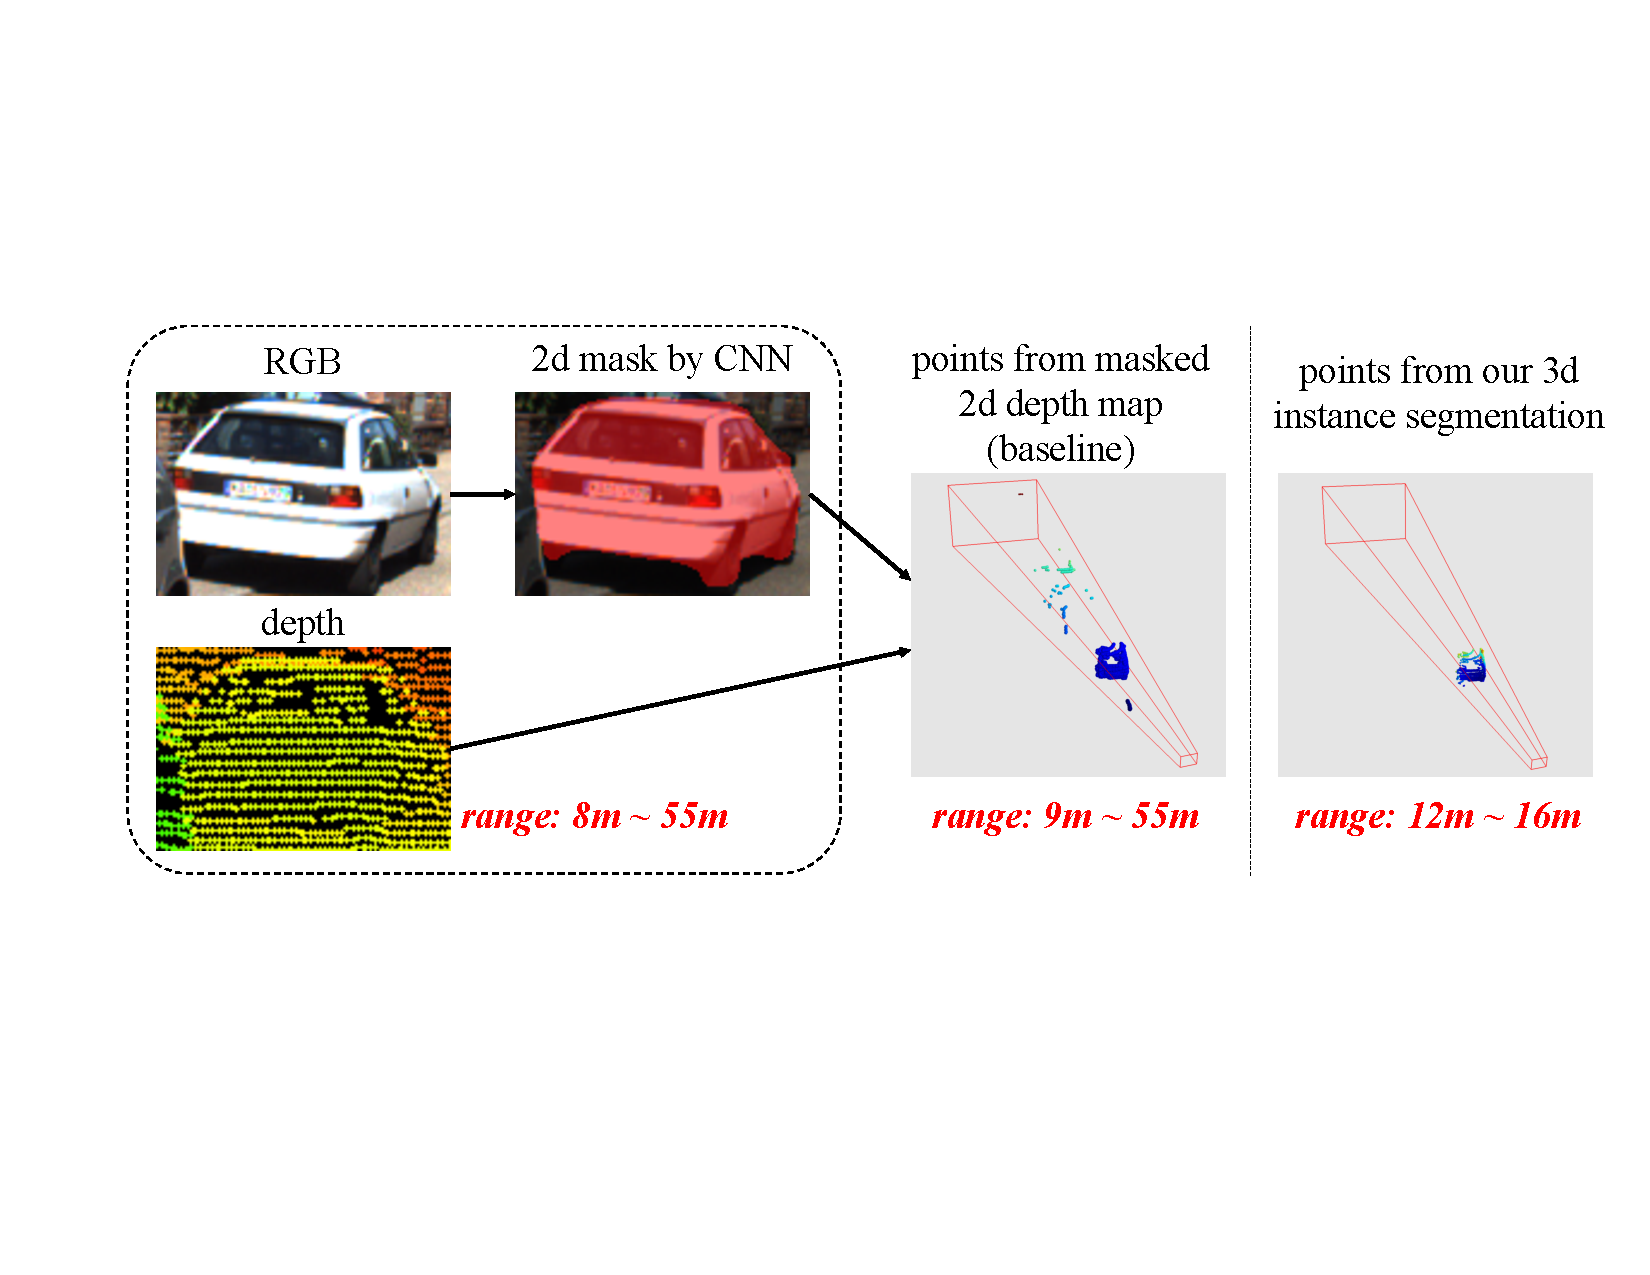
\includegraphics[width=0.96\linewidth]{fig/mask2d3d.pdf}
    \caption{\textbf{Comparisons between 2D and 3D masks.} We show a typical 2D region proposal from KITTI val set with both 2D (on RGB image) and 3D (on frustum point cloud) instance segmentation results. The red numbers denote depth ranges of points.}
    \label{fig:mask2d3d}
\end{figure}


% \begin{table}[h!]
% \centering
% \label{tab:corner_loss}
% \begin{tabular}{c|cc}
% \hline
% Loss type                                & $\gamma$ & Accuracy \\ \hline
% multi-bin                                & -        & 71.8    \\ 
% multi-bin norm                           & -        & 72.2    \\ \hline
% \multirow{4}{*}{multi-bin norm + corner} & 0.1      & 72.4    \\
%                                          & 1        & 73.2    \\
%                                          & 10       & \textbf{74.3}    \\
%                                          & 50       & 73.9    \\ \hline
% \end{tabular}
% \caption{3D box loss and formulation (corner only, loss weight). \rqi{Consider using a figure for this section}}
% \end{table}


% \paragraph{Effects of PointNet architectures.} Table~\ref{tab:v1v2} compares PointNet~\cite{qi2017pointnet} (v1) and PointNet++~\cite{qi2017pointnetplusplus} (v2) architectures for instance segmentation and amodal box estimation. The v2 model outperforms v1 model on both tasks because 1) v2 model learns hierarchical features that are richer and more generalizable; 2) v2 model uses multi-scale feature learning that adapts to varying point densities. Note that the ours (v1) model reported in Table~\ref{tab:kitti_test_3d_detection} corresponds to first row of Table~\ref{tab:v1v2} while the ours (v2) links to the last row.

% \begin{table}[h!]
% \centering
% \begin{tabular}{cc|cc}
% \hline
% seg net & box net & seg acc. & box acc. \\ \hline
% v1   & v1   & 90.6 & 74.3  \\
% v2   & v1   & \textbf{91.0} & 74.7 \\
% v1   & v2   & 90.6 & 76.0 \\
% v2   & v2   & \textbf{91.0}  & \textbf{77.1} \\ \hline
% \end{tabular}
% \caption{\textbf{Effects of PointNet architectures.} Metric is 3D box estimation accuracy with IoU=0.7.}
% \label{tab:v1v2}
% \end{table}

%Effects of adding image features (sensor fusion)
%Effects of quality of 2d detector/proposals

%% QUALITATIVE RESULTS
\vspace{-.16in}
\subsection{Qualitative Results and Discussion}
\label{sec:exp_viz}
% \begin{enumerate}
%     \item Both success and failure cases
%     \item Step by step visualization show 2D box, frustum, 3D binary segmentation, 3D object center estimation
% \end{enumerate}
In Fig.~\ref{fig:results} we visualize representative outputs of our frustum PointNet model. We see that for simple cases of non-occluded objects in reasonable distance (so we get enough number of points), our model outputs remarkably accurate 3D instance segmentation mask and 3D bounding boxes. Second, we are surprised to find that our model can even predict correctly posed \emph{amodal} 3D box from partial data (e.g. parallel parked cars) with few points. Even humans find it very difficult to annotate such results with point cloud data only. Third, in some cases that seem very challenging in images with lots of nearby or even overlapping 2D boxes, when converted to 3D space, the localization becomes much easier (e.g. P11 in second row third column).

On the other hand, we do observe several failure patterns, which indicate possible directions for future efforts.
The \emph{first} common mistake is due to inaccurate pose and size estimation in a sparse point cloud (sometimes less than 5 points). We think image features could greatly help esp. since we have access to high resolution image patch even for far-away objects.
The \emph{second} type of challenge is when there are multiple instances from the same category in a frustum (like two persons standing by). Since our current pipeline assumes a single object of interest in each frustum, it may get confused when multiple instances appear and thus outputs mixed segmentation results. This problem could potentially be mitigated if we are able to propose multiple 3D bounding boxes within each frustum.
\emph{Thirdly}, sometimes our 2D detector misses objects due to dark lighting or strong occlusion.  Since our frustum proposals are based on region proposal, no 3D object will be detected given no 2D detection. However, our 3D instance segmentation and amodal 3D box estimation PointNets are not restricted to RGB view proposals. As shown in the supplementary, the same framework can also be extended to 3D regions proposed in bird's eye view.



% \subsection{Runtime}
% \label{sec:runtime}
% In Table~\ref{tab:runtime}, we show decomposed runtime cost for our frustum PointNets (v1 and v2). The evaluation is based on TensorFlow with a NVIDIA GTX 1080 and a single CPU core. While for v1 model frustum proposal (with CNN and backprojection) takes the majority time, for v2 model since PointNet++~\cite{qi2017pointnetplusplus} models with multi-scale grouping is used, computation bottleneck shifts to instance segmentation. 

% CNN model has size 28 MB. v1 PointNets have size 19MB. v2 PointNets have size 22MB. SO the total size is 47MB for v1 model and 50MB for v2 model.

% \begin{table}[h!]
% \small
% \centering
% \begin{tabular}{c|ccc|c}
% \hline
% Model & Frustum Proposal & 3D Seg &  Box Est. & Total \\ \hline
% v1 & 60 ms & 18 ms & 10 ms & 88 ms \\ 
% v2 & 60 ms & 88 ms & 19 ms & 167 ms \\ \hline
% \end{tabular}
% \caption{\textbf{3D detector runtime.} Thirty-two region proposals used for frustum-based PointNets. 1,024 points are used for instance segmentation and 512 points are used for box estimation.}
% \label{tab:runtime}
% \end{table}